\documentclass[tikz]{standalone}
\usepackage{tikz}
\usetikzlibrary{positioning}
\usetikzlibrary{calc}

\begin{document}

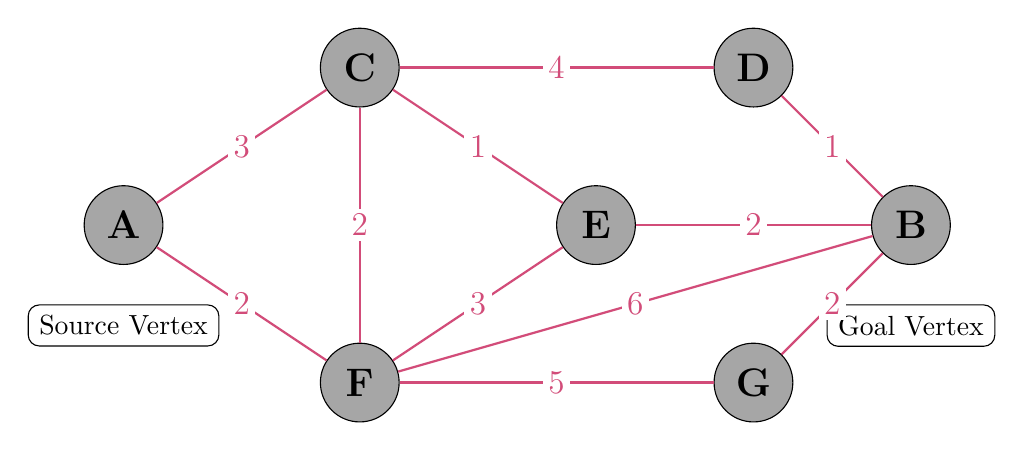
\begin{tikzpicture}[
    node distance=3cm,
    vertex/.style={circle, draw, fill=gray!70, minimum size=1cm, font=\Large\bfseries},
    edge/.style={draw, thick, color=purple!70},
    weight/.style={fill=white, inner sep=2pt, font=\large}
]

% Define node positions
\node[vertex] (A) at (-4, 0) {A};
\node[vertex] (C) at (-1, 2) {C};
\node[vertex] (F) at (-1, -2) {F};
\node[vertex] (E) at (2, 0) {E};
\node[vertex] (D) at (4, 2) {D};
\node[vertex] (B) at (6, 0) {B};
\node[vertex] (G) at (4, -2) {G};

% Add source vertex label
\node[below=0.5cm of A, draw, fill=white, rounded corners, inner sep=4pt] {Source Vertex};

% Add goal vertex label
\node[below=0.5cm of B, draw, fill=white, rounded corners, inner sep=4pt] {Goal Vertex};

% Draw edges with weights
\draw[edge] (A) -- (C) node[weight, midway] {3};
\draw[edge] (A) -- (F) node[weight, midway] {2};
\draw[edge] (C) -- (D) node[weight, midway] {4};
\draw[edge] (C) -- (E) node[weight, midway] {1};
\draw[edge] (C) -- (F) node[weight, midway] {2};
\draw[edge] (E) -- (F) node[weight, midway] {3};
\draw[edge] (E) -- (B) node[weight, midway] {2};
\draw[edge] (F) -- (B) node[weight, midway] {6};
\draw[edge] (D) -- (B) node[weight, midway] {1};
\draw[edge] (B) -- (G) node[weight, midway] {2};
\draw[edge] (F) -- (G) node[weight, midway] {5};

\end{tikzpicture}

\end{document} 